\section{Risultati}
\subsection{Immagini satellitari}
In questa sezione sono riportati i risultati ottenuti dal calcolo dell'indice NDWI8A e dalla sua differenza per due periodi temporali differenti.\\
Nella figura \ref{fig:ndwi8a_18_19} è indicata la differenza tra i periodi 2018 e 2019. Si può notare come, nelle aree maggiormente colorate di rosso/giallo, ci sia stata una maggiore severità al disturbo di vento.\\
Mediante interrogazione del raster è possibile notare come la variazione massima sia stata di 0.38 e quella media di 0.037.\\ 
Nella figura \ref{fig:ndwi8a_18_25} è invece indicata la differenza di NDWI8A tra il 2018 e 2025. In questo caso, la variazione massima di NDWI8A tra i due anni è stata di 0.23, mentre quella media di 0.0002.\\
Infatti, è evidente la differenza tra le condizioni 2018-2019 e 2018-2025.\\
Un motivo plausibile di questa variazione risiede nella presenza di rinnovazione al suolo, che porta ad un aumento dell'indice NDWI8A nel periodo 2025.\\
Un'altra motivazione plausibile della differenza nei risultati tra i due momenti risiede nella qualità delle immagini telerilevate: infatti nel 2019 c'è stata una maggiore registrazione di aree affette da copertura nuvolosa, che possono aver modificato il rilievo da parte del satellite. 
\begin{figure}[H]
    \centering
    \includegraphics[width=0.7\textwidth]{immagini/ndwi8a_18_19.pdf}
    \caption{Differenza di NDWI8A tra le estati del 2018 e del 2019.}    
    \label{fig:ndwi8a_18_19}
\end{figure}
\begin{figure}[H]
    \centering
    \includegraphics[width=0.7\textwidth]{immagini/ndwi8a_18_25.pdf}
    \caption{Differenza di NDWI8A tra le estati del 2018 e del 2025.}    
    \label{fig:ndwi8a_18_25}
\end{figure}
\subsection{Area non colpita}
Successivamente alla raccolta dei dati, è possibile applicare le formule precedentemente esposte, e ricavare i risultati del relativo rilievo (tabella \ref{tab:risultati_novaia}).
\begin{table}[H] \centering
\caption{Valori dendrometrici di densità della particella di bosco non soggetta a schianti da vento.}
\label{tab:risultati_novaia}
\begin{tabular}{cccc}
    \toprule
Classi diam. (cm) & Freq. (n) & Freq. (n/ha) \\
    \midrule
10 & 1 & 31.85 \\
15 & 1 & 31.85 \\
20 & 2 & 63.69 \\
25 & 1 & 31.85 \\
30 & 2 & 63.69 \\
35 & 1 & 31.85 \\
40 & 1 & 31.85 \\
50 & 1 & 31.85 \\
60 & 1 & 31.85 \\
65 & 1 & 31.85 \\
80 & 1 &31.85 \\
\bottomrule
\end{tabular}
\end{table}
\begin{table}[H] \centering
\caption{Valori dendrometrici di densità della particella di bosco non soggetta a schianti da vento.}
\begin{tabular}{cccccc}
    \toprule
$G_{tot}$ ($m^2$) & $G_{tot}$ ($m^2/ha$) & N & $N/ha$ &Diametro medio (m) & Altezza media (m) \\
   % \midrule
1.842 & 58.68 & 13 & 414 & 0.43 & 27.32 \\
\bottomrule
\end{tabular}
\end{table}
\begin{figure}[H]
    \centering
    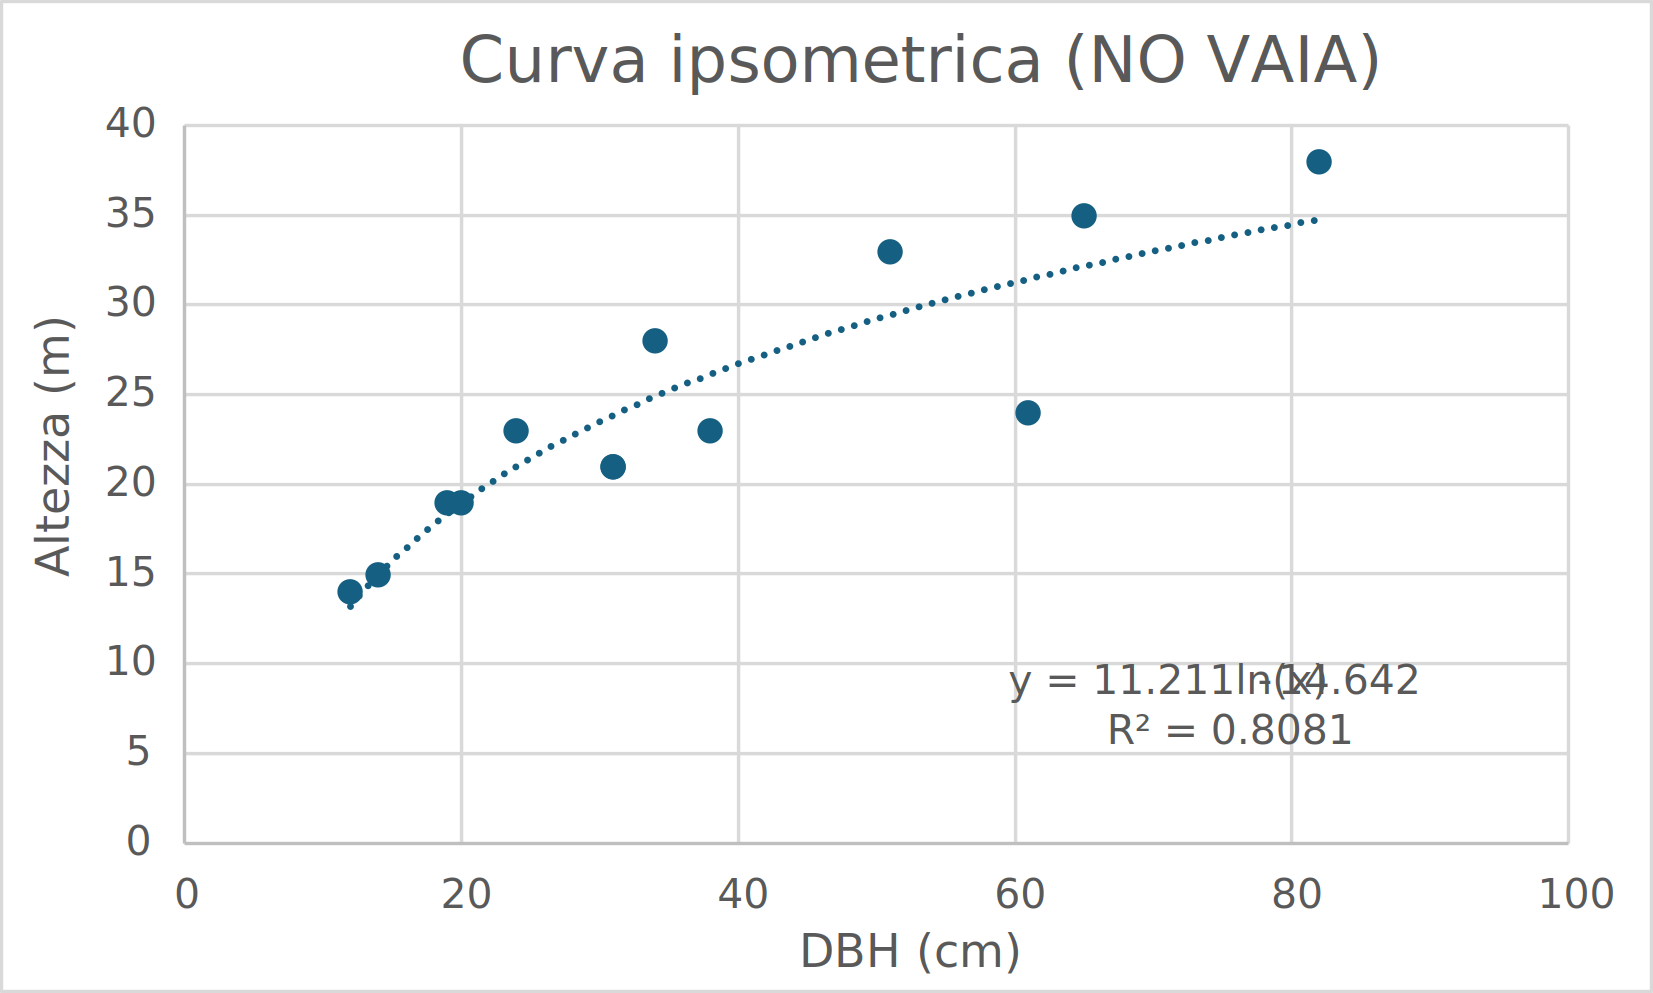
\includegraphics[width=0.8\textwidth]{immagini/curva_ipsometrica_novaia.png}
    \caption{Curva ipsometrica dell'area di saggio (comprendente quindi più specie arboree).}    
    \label{fig:curva_ipsometrica_novaia}
\end{figure}
\subsection{Aree colpite}
Dai rilievi svolti nelle aree soggette a schianti da vento, è possibile estrarre due parametri importanti, ovvero la valutazione della necromassa ancora presente (tabella \ref{tab:necromassa}) e la rinnovazione in evoluzione (\cref{fig:copertura_excel}).\\
È doveroso far presente che la necromassa misurata è il risultato di operazioni selvicolturali applicate successivamente all'evento Vaia. Pertanto, è ovvio che nel periodo immediatamente successivo alla perturbazione, il materiale a terra fosse ben superiore.
\begin{table}[H] \centering
\caption{Valori di necromassa misurati nelle singole aree di saggio.}
\label{tab:necromassa}
\begin{tabular}{cccc}
    \toprule
 & Area 2 & Area 4 & Area 6 \\
    \midrule
Vol. ($m^3$) & 1.43 & 0.96 &0.91 \\
Vol. ($m^3/ha$) & 181.60 & 121.96 & 116.00\\
Stump ($n/ha$) & 255& 637& 892\\
\bottomrule
\end{tabular}
\end{table}
\begin{figure}[H]
    \centering
    \includegraphics[width=0.7\textwidth]{immagini/copertura_excel.png}
    \caption{Grafico indicante la componente di copertura nelle singole aree di saggio.}    
    \label{fig:copertura_excel}
\end{figure}
\begin{figure}[H]
    \centering
    \includegraphics[width=0.7\textwidth]{immagini/necromassa_ndwi.pdf}
    \caption{Quantità di necromassa ipotizzata ($m^3/ha$), in confronto alla severità registrata tra il periodo 2018 e 2019 (mediante NDWI8A). I punti indicano le aree di saggio colpite dall'evento Vaia.}    
    \label{fig:ndwi8a_18_25}
\end{figure}
\begin{figure}[H]
    \centering
    \includegraphics[width=0.7\textwidth]{immagini/copertura_ndwi.pdf}
    \caption{Copertura del suolo valutata, in confronto alla severità registrata tra il periodo 2018 e 2019 (mediante NDWI8A).}    
    \label{fig:copertura_ndwi}
\end{figure}